\chapter{A new approach to STM analysis}
Conventional methods in analyzing grid maps from STM measurements face multiple fundamental  challenges. Recently, thanks to the maturation of optimization algorithms, a convolution data model for STM datasets was proposed by Cheung et al.\cite{cheungDictionaryLearningFouriertransform2020} and shows great potential. However,  despite its success in addressing some of the challenges, key shortcomings exist that prevent it being useful in most of the specimens studied by STM. In this chapter, we introduce a more general model that extends the convolution framework, we then showcase its performance with various benchmark tests, and apply it to real STM data as an illustration.  

\section{Challenges of the conventional analysis methods}
In this section, I will briefly introduce the conventional analysis methods used in the field, two fundamental challenges faced with the current method, and discuss the existing approaches to address these challenges and their limitations. 

%todo: make changes to clarify the things I want to say with the grant claims.
Fundamentally, the data obtained from experiments—particularly in techniques like quasiparticle interference scanning tunneling microscopy (QPI-STM)—are not direct representations of the underlying physical mechanisms. Instead, they are convolutions of the interpretable signatures we aim to extract (such as interference patterns or defect-induced modulations) with a range of additional contributions—instrument response, scanning junction variations, and noise. This complexity means that careful data analysis is often essential to uncover the true physical insights. Among conventional methods, the Fourier Transform (FT) is widely used to extract characteristic wavelengths and relate them to theoretical predictions across different systems \cite{ardiniHighthroughputMultimodalWidefield2023}\cite{jaffeDifferenceFourierAnalysis1987}
\noindent \cite{sciuttoFTNIRMicroscopyAdvanced2014}\cite{kimotoAssessmentLowervoltageTEM2012}.

However, FT has notable limitations, especially when applied to more complex or less ideal datasets. In systems with nearly perfect periodicity, FT produces sharp, interpretable peaks. But in more realistic scenarios—where signals include aperiodic features such as randomly distributed defects —the FT tends to produce blurred spectra, diffuse speckles, and loss of phase information. This can severely hinder the interpretability of the results and mask the very features researchers are trying to study. While these challenges are particularly evident in QPI-STM, similar issues arise in other imaging and spectroscopic techniques where signal complexity or disorder is present\cite{Bonnet 1997} \cite{Draijer 2009}.

In the context of QPI analysis, these limitations give rise to two specific and critical problems we aim to address: the speckle problem and the demixing problem. In the following, we will define these challenges more formally and introduce a convolution-based data model designed to overcome them.
\begin{figure}
	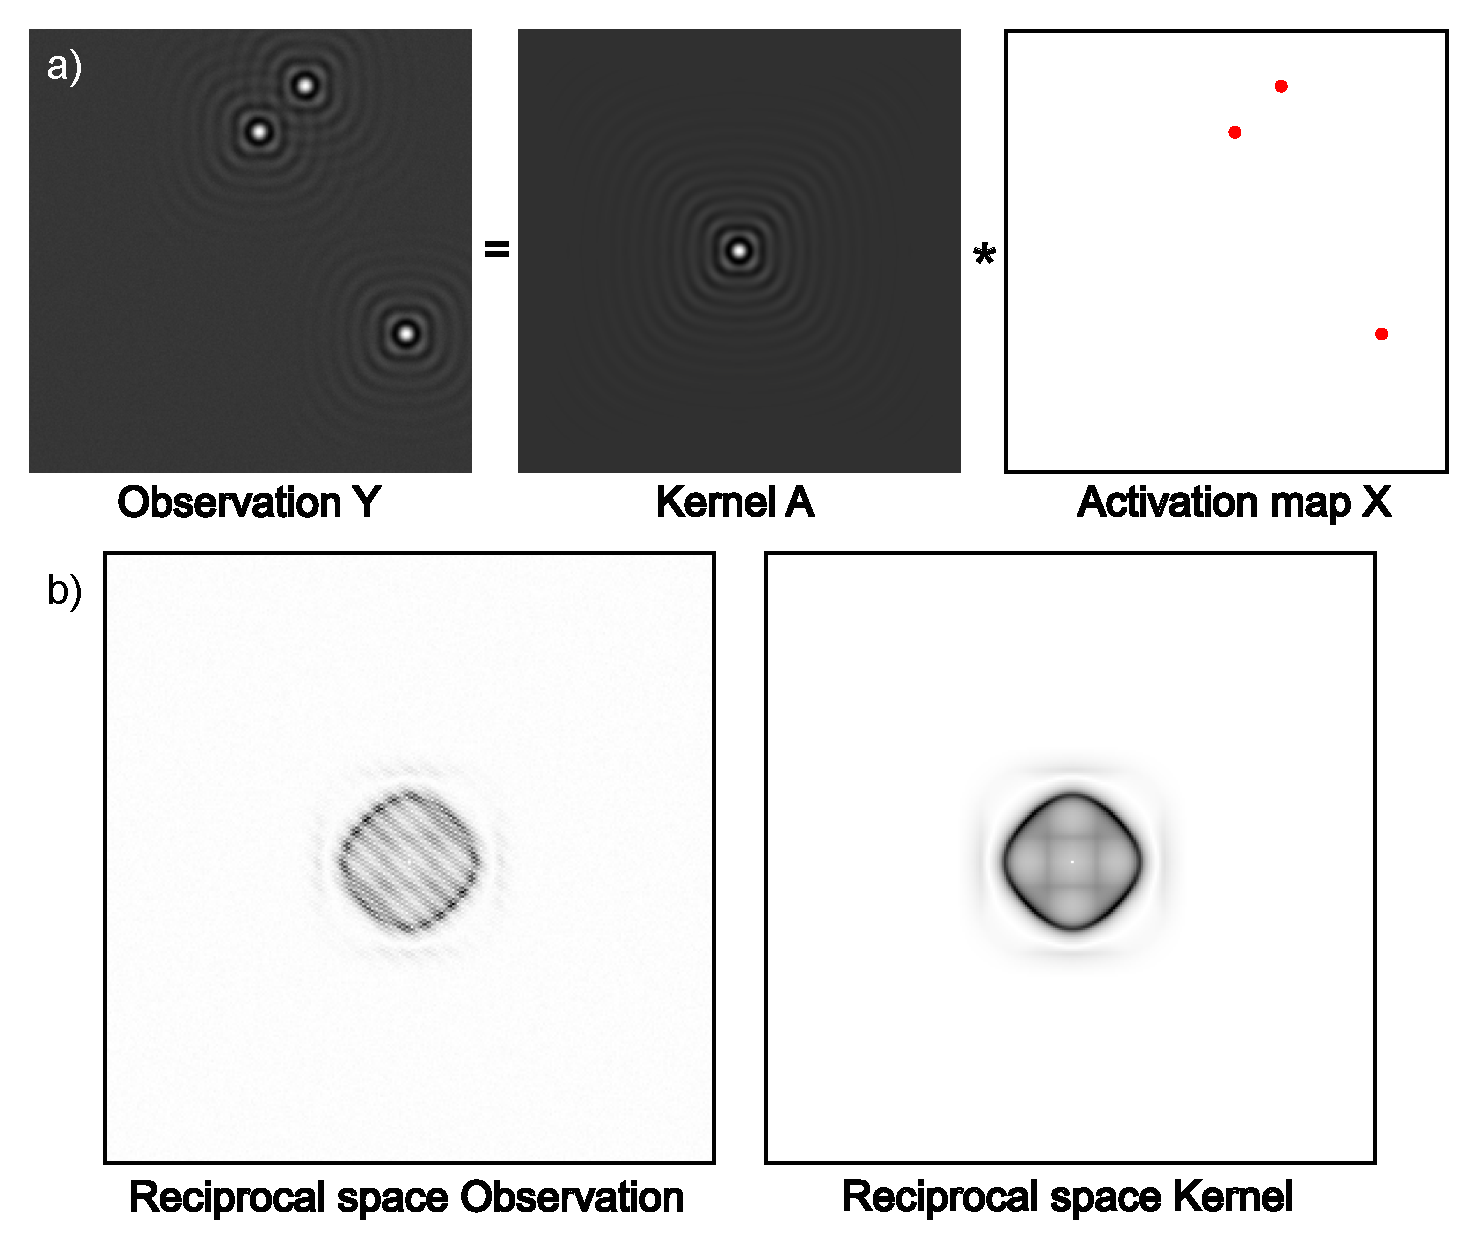
\includegraphics[width= \textwidth]{Ch6_deconvolution.pdf} 
	\centering
	\caption{Illustration of the observation generation process and the speckle problem. a) The QPI-STM data generation process can be seen as the convolution between the QPI pattern of a defect (the kernel A) and its location map (the activation map X). We can take the Fourier transform of the observation and the kernel, respectively and get b); clear speckle is presented in the FT-observation, which hindered the desired pattern of $\delta\rho_0$ as presented on the right}
	\label{fig:ch6_decon}
\end{figure}

\subsection{The Speckle problem}
As introduced in the end of Ch5 and theorized explicitly in Equation \ref{eq.539}, when we take \ac{FT} of the grid map on multiple occurrence of defects, we get speckle on the \ac{FT-STS}. The speckle acts as a mask on top of the QPI pattern, thus making the intrinsic pattern hard to interpret. Therefore, to address the challenge of speckle is to disentangle the spatial information from the \ac{QPI} pattern, and this can be formulated mathematically as a deconvolution problem. 

\par \noindent Recall that we can write the modulation of \ac{LDOS} $\delta \rho$ from multiple defects as:
\begin{equation}
	\delta \rho(\mathbf{x}, \omega) = \sum_{j=1}^{N}c_j \cdot \delta \rho_0(\mathbf{x}-\mathbf{x_j},\omega),
\end{equation}
\noindent where $\delta \rho_0$ is the \ac{LDOS} modulation from individual defect located at at $\mathbf{x_j}$. We can further separate the spatial information by utilizing a Kronecker delta $\Delta(\mathbf{u})$, so that $\Delta(\mathbf{u})=1$ if $\mathbf{u} = 0$, and $\Delta(\mathbf{u})=0$ elsewhere: 
\begin{equation}
	\sum_{j=1}^{N}c_j \cdot \delta \rho_0(\mathbf{x}-\mathbf{x_j},\omega) = \sum_{\mathbf{u}} \delta \rho_0(\mathbf{x}-\mathbf{u},\omega)\cdot(\sum_{j=1}^{N} c_j \cdot \Delta(\mathbf{u-x_j})).
\end{equation}
\noindent We can then construct a convolution sum between the individual \ac{QPI} pattern and the spatial information by defining a defect location function $D(\mathbf{x}) \equiv \sum_{j=1}^{N} c_j \cdot \Delta(\mathbf{u-x_j})$, we have: 
\begin{equation}
	\delta \rho(\mathbf{x}, \omega) =  \sum_{\mathbf{u}} \delta \rho_0(\mathbf{x}-\mathbf{u},\omega)\cdot D(\mathbf{u}) = (\delta \rho_0 *D)(\mathbf{x}, \omega).
\end{equation}

We illustrate this convolution in Fig. \ref{fig:ch6_decon} a); first, we use $\delta \rho_0$ simulated in Ch.5.2 as the \ac{QPI} pattern from an single defect, we then randomly generate a binary defect location map given a defect density, and use the convolution sum to construct an observation. To unify the language, we will now refer to the single defect \ac{QPI} pattern as a kernel, denoted as A, and the defect location map as an activation map, denoted as X; thus, we can express our observation as $Y = A * X$. Then, we follow the conventional approach and take \ac{FT} of both the observation Y and the kernel A As shown in panel b), the \ac{FT} of Y shows clear speckle compared to the \ac{FT} of the kernel.

There have been few attempts made to address the speckle, partially because speckle are less disruptive at higher defect density, as illustrated in the Figure. \ref{fig:ch5_changephasenoise}. Another "mitigation" is through brute force and finding an isolated defect, which is possible in low defect concentration materials but less so with dense defects. Recently, due to advancement in machine learning, researchers treated speckle as a source of noise and try to address it with self-supervised algorithms like Noise2Self \cite{kuijfSelfsupervisedLearningDenoising2025}, this present good performance in synthetic data, however, the blackbox nature of the machine learning algorithm makes it hard to tell the performance in real data, as the denoising process is hard to interpret. Another line of effort is the development of deconvolution algorithms, which includes the SBD-STM algorithm presented by Cheung et al \cite{cheungDictionaryLearningFouriertransform2020}, which inspired this body of work.
 

\subsection{The Demixing problem}
Materials normally exhibit multiple types of defects, and these defects could present different scattering features. QPI measurements are especially powerful on materials that possess distinct scattering features on different defects, such as the sign variation of the superconducting order parameter \cite{chiSignInversionSuperconducting2014}, and the spin and orbital texture of topological bands \cite{yinProbingTopologicalQuantum2021}\cite{butlerQuasiparticleInterferenceZrSiS2017}. 

To access impurity-dependent scattering information requires demixing different defects from a single grid map. However, there are only limited approaches to analyze and disentangle defect-dependent scattering features. The most common approach is to acquire grid spectroscopy on isolated defects, or to crop around individual defects in larger grid maps if the isolated defect is hard to find. One example is the Dirac semimetal ZrSiS, where the interference patterns around impurities located on the Zr and S sublattice sites scatter differently \cite{butlerQuasiparticleInterferenceZrSiS2017}; As shown in Figure. \ref{fig:ch6_ZrSiS}, conventional \ac{FT} displays a mixture of the scattering features, which are disentangled through inspecting the \ac{FT} of cropped grid spectroscopy around individual defects. 

There are 2 primary shortcomings with this approach: one is due to a small spatial range of the cropping, the resolution in q-space is very much limited, making it hard to resolve features with higher frequencies. Second is that the cropped area could still preserve features from other defect sources, this is particularly problematic when we have quasiparticles with longer lifetime. They induce weakly damped standing waves whose decaying tail could easily spread tens of unit cells, making it hard to avoid when cropping. 

\begin{figure}
	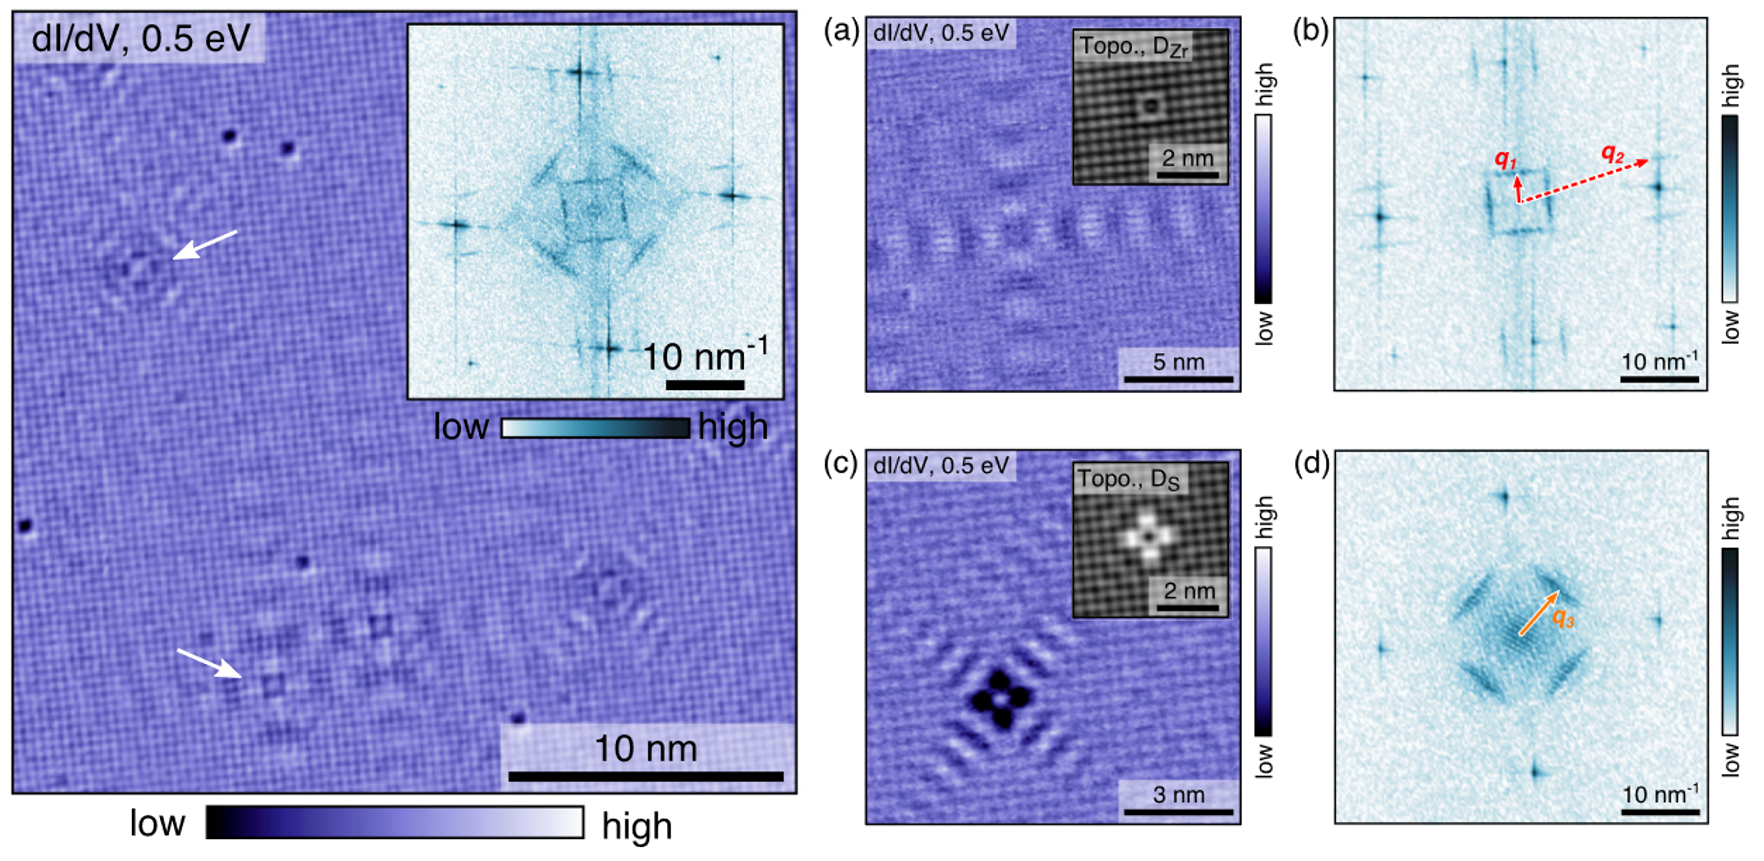
\includegraphics[width= \textwidth]{ZrSiS.png} 
	\centering
	\caption[Selective band scattering in ZrSiS]{\textbf{Selective band scattering in ZrSiS}. On the left, \ac{FT} of the whole grid map sees the band scattering. a)-d): The selective band scattering of different defects can be accessed by cropping around the individual defect QPI pattern and take the \ac{FT}/ However, due to the small spatial range of the cropped image, the q-space maps have limited resolution.}
	\label{fig:ch6_ZrSiS}
\end{figure}

\begin{figure}
	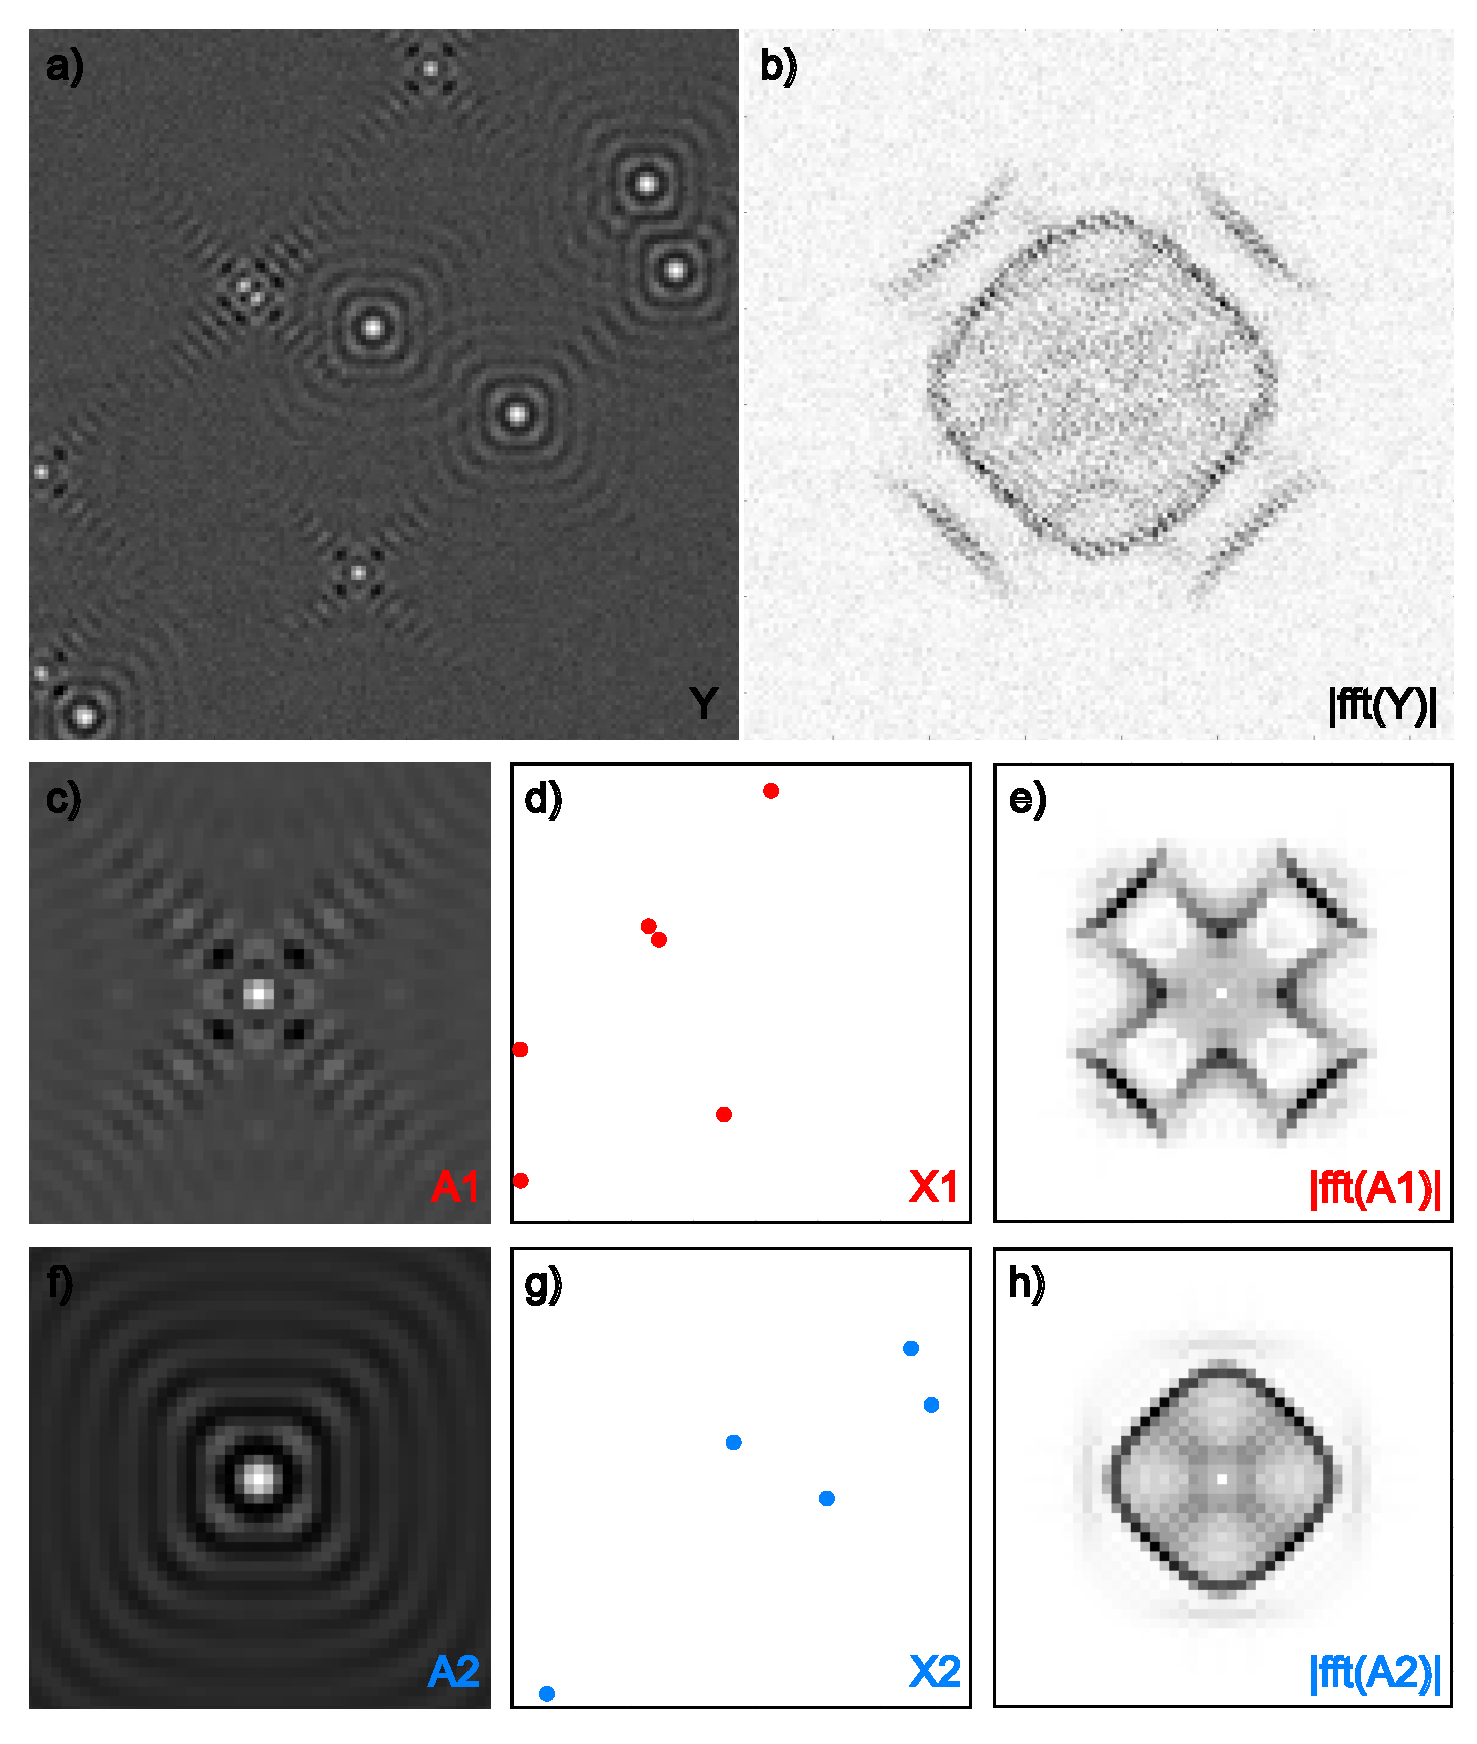
\includegraphics[width= \textwidth]{Ch6_demixing.pdf} 
	\centering
	\caption{Demixing as an inverse data generation process. Given the observation 
		$Y$ in (a), the goal is to reconstruct QPI patterns around individual impurities(kernels), as shown in (c) and (f). By applying a Fourier transform to each reconstructed kernel, we can isolate impurity-dependent scattering features, illustrated in (e) and (h).}
	\label{fig:ch6_demix}
\end{figure}

We now use our synthetic data to better illustrate the demixing problem. We simulate 2 \ac{QPI} patterns from 2 distinct defects with kernel choices A1 and A2 as shown in Fig. \ref{fig:ch6_demix} c) and d); We then define their activation maps X1 and X2 in d) and g). By summing up the convolutions between 2 kernels and their corresponding activation maps, we can obtain an observation Y in a). We express the above observation generation process as:

\begin{equation}
	Y = A1 * X1 + A2 * X2 + \beta, 
\end{equation}
where $\beta$ is the added noise determined by a pre-defined signal-to-noise ratio.

The demixing problem is the inverse of the observation generation process: given the observation Y, our goal is to reconstruct A1, A2. This means that in reciprocal space, rather than working with entangled and less informative data like (b), we can recover disentangled QPI patterns from individual defect types, as shown in (e) and (h), which are also free from speckle. Lastly, we extend the above formulation with multiple types of different defects, then at arbitrary energy $\omega$, we have: 

\begin{equation}
	\label{eq:demixing}
	Y_{\omega} = \sum_d ( A_{d,{\omega}} * X_d) + \beta. 
\end{equation} 





\section{Experimental QPI measurement}
Realspace \ac{QPI} signals are obtained by taking the grid map experiment on a region that presents \ac{QPI} patterns. In this section we will briefly explore \ac{QPI} measurement in the \ac{STM} experiment, more specifically, we will introduce the factors that dictate \ac{QPI} quality, discuss how to choose proper parameters that result in a good \ac{QPI} measurement, and finally we will present a specific challenge called the phase noise, which motivates our work in the next chapter.


\subsection{QPI measurement and quality}
As mentioned in Ch.2, taking a grid map is very involved. A successful grid map requires both an ideal instrumental setup and a set of proper measurement parameters based on the understanding of the targeting material. 

The key objective of an ideal instrumental setup is to create a stable environment and lower the system noise; as we discussed in Ch.2, this involves minimizing the noise from mechanical vibration, temperature fluctuation, and electronic instability of the system and maintaining a stable tip-surface tunneling junction. 

A grid map is defined by a $N\times N$ (assuming square) grid on a targeted area of $L \times L$ $nm^2$, this provides a spatial resolution $\Delta L = \frac{L}{N}$; In reciprocal space, this set up gives a range $Q = \frac{2 \pi}{\Delta L}$ with resolution $\Delta Q = \frac{2\pi}{L}$, the energy range and resolution is defined by the setting of the single-point spectroscopy performed on every grid point. 

A set of proper parameters for \ac{QPI} measurement aims to extract the most amount of information with the highest level of resolution given the constraints of the system. The most important constraint is the limiting cryogenic holding time. This puts a ceiling on the grid map run time, while different systems vary; typically, the cryogenic holding time is a fraction of a week. Within the boundary of the run time, we usually aim for a grid with a fine reciprocal resolution $\Delta Q$ and a reasonable reciprocal range $Q$, corresponding to a large field of view $L$ and a reasonable $\Delta L$. It is intuitive to have a proper size of reciprocal range $Q$ that is not infinitely large, as most of the q-space features reside within the Bragg peaks, exemplified by Fig. \ref{fig:ch5_ldos} c). But we also do not want the field of view $L$ to be too large, this is because in real experiments with finite noise level, the featured \ac{QPI} pattern has a finite lifetime and its intensity will dive under the noise at some cutoff distance $r_{cutoff}$ from the defect center; Thus, a field of view larger than the cutoff distance will instead decrease the signal to noise ratio. We illustrate cutoff distances in systems with different noise levels in Fig. \ref{fig:ch5_cutoff}. The noise level is set to be noiseless, SNR = 10, and SNR = 1.2, respectively; given the noise level shown in the green dotted line, we identify the furthest signal peak higher than the noise level and place a blue vertical line there. These vertical lines indicate the cutoff distances; and we can see with increasing noise level, $r_{cutoff}$ drops, and thus the optimal field of view should also drop.  

\begin{figure}
	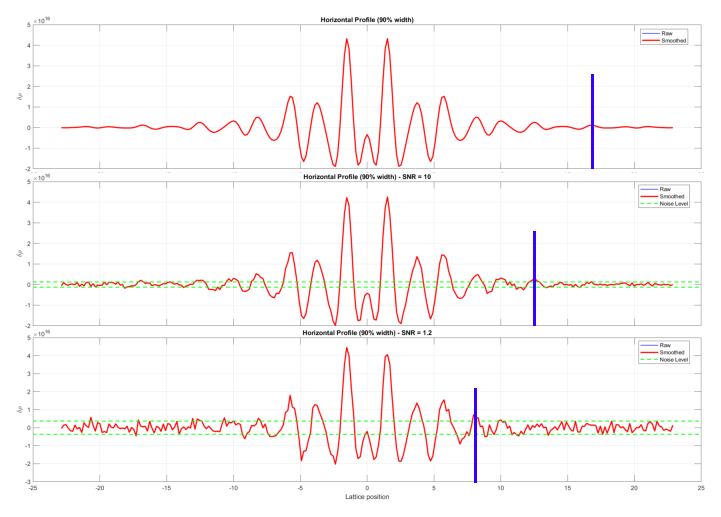
\includegraphics[width=\textwidth]{Ch5_fieldofview.pdf} 
	\centering
	\caption{Cutoff distances of QPI patterns with different signal-to-noise ratios. Three Horizontal Line profiles on $\delta\rho(\textbf{x}, E=0.45eV)$ with the noise of various levels. a) has no noise applied; b), c) have Gaussian noises applied with SNR = 10 and 1.2, respectively. Here the signal strength is defined as the variance of the noiseless $\delta\rho(\textbf{x}, E=0.45eV)$, see a) of Fig. \ref{fig:ch5_single_scattering}.}
	\label{fig:ch5_cutoff}
\end{figure}


\subsection{multi-defect QPI pattern and phase noise}
\ac{QPI} patterns present themselves around defects. While an ideal \ac{QPI} measurement is performed on isolated defects in a large field of view, it is normally difficult to find such a case. In real experiments, grid maps are usually taken on areas with multiple defects; this causes interference between the \ac{QPI} patterns originating from different defects, as hinted by Ch.5.2.4 when discussing Fig. \ref{fig:ch5_multi_scattering}.

This is problematic when we try to interpret the \textbf{q}-space \ac{QPI} map. As illustrated in Fig. \ref{fig:ch5_phasenoise}, when we have multiple defects scattered in the field of view, we start to see some noise patterns associated with the spatial distribution of the defects, as we can see by comparing c) and e), we see that with nothing but the relative locations of the defects changed, the corresponding \textbf{q}-space \ac{QPI} maps possess different noise patterns. This effect is called phase noise; it hinders our ability to analyze the underlying quasiparticle scattering process. 

\begin{figure}
	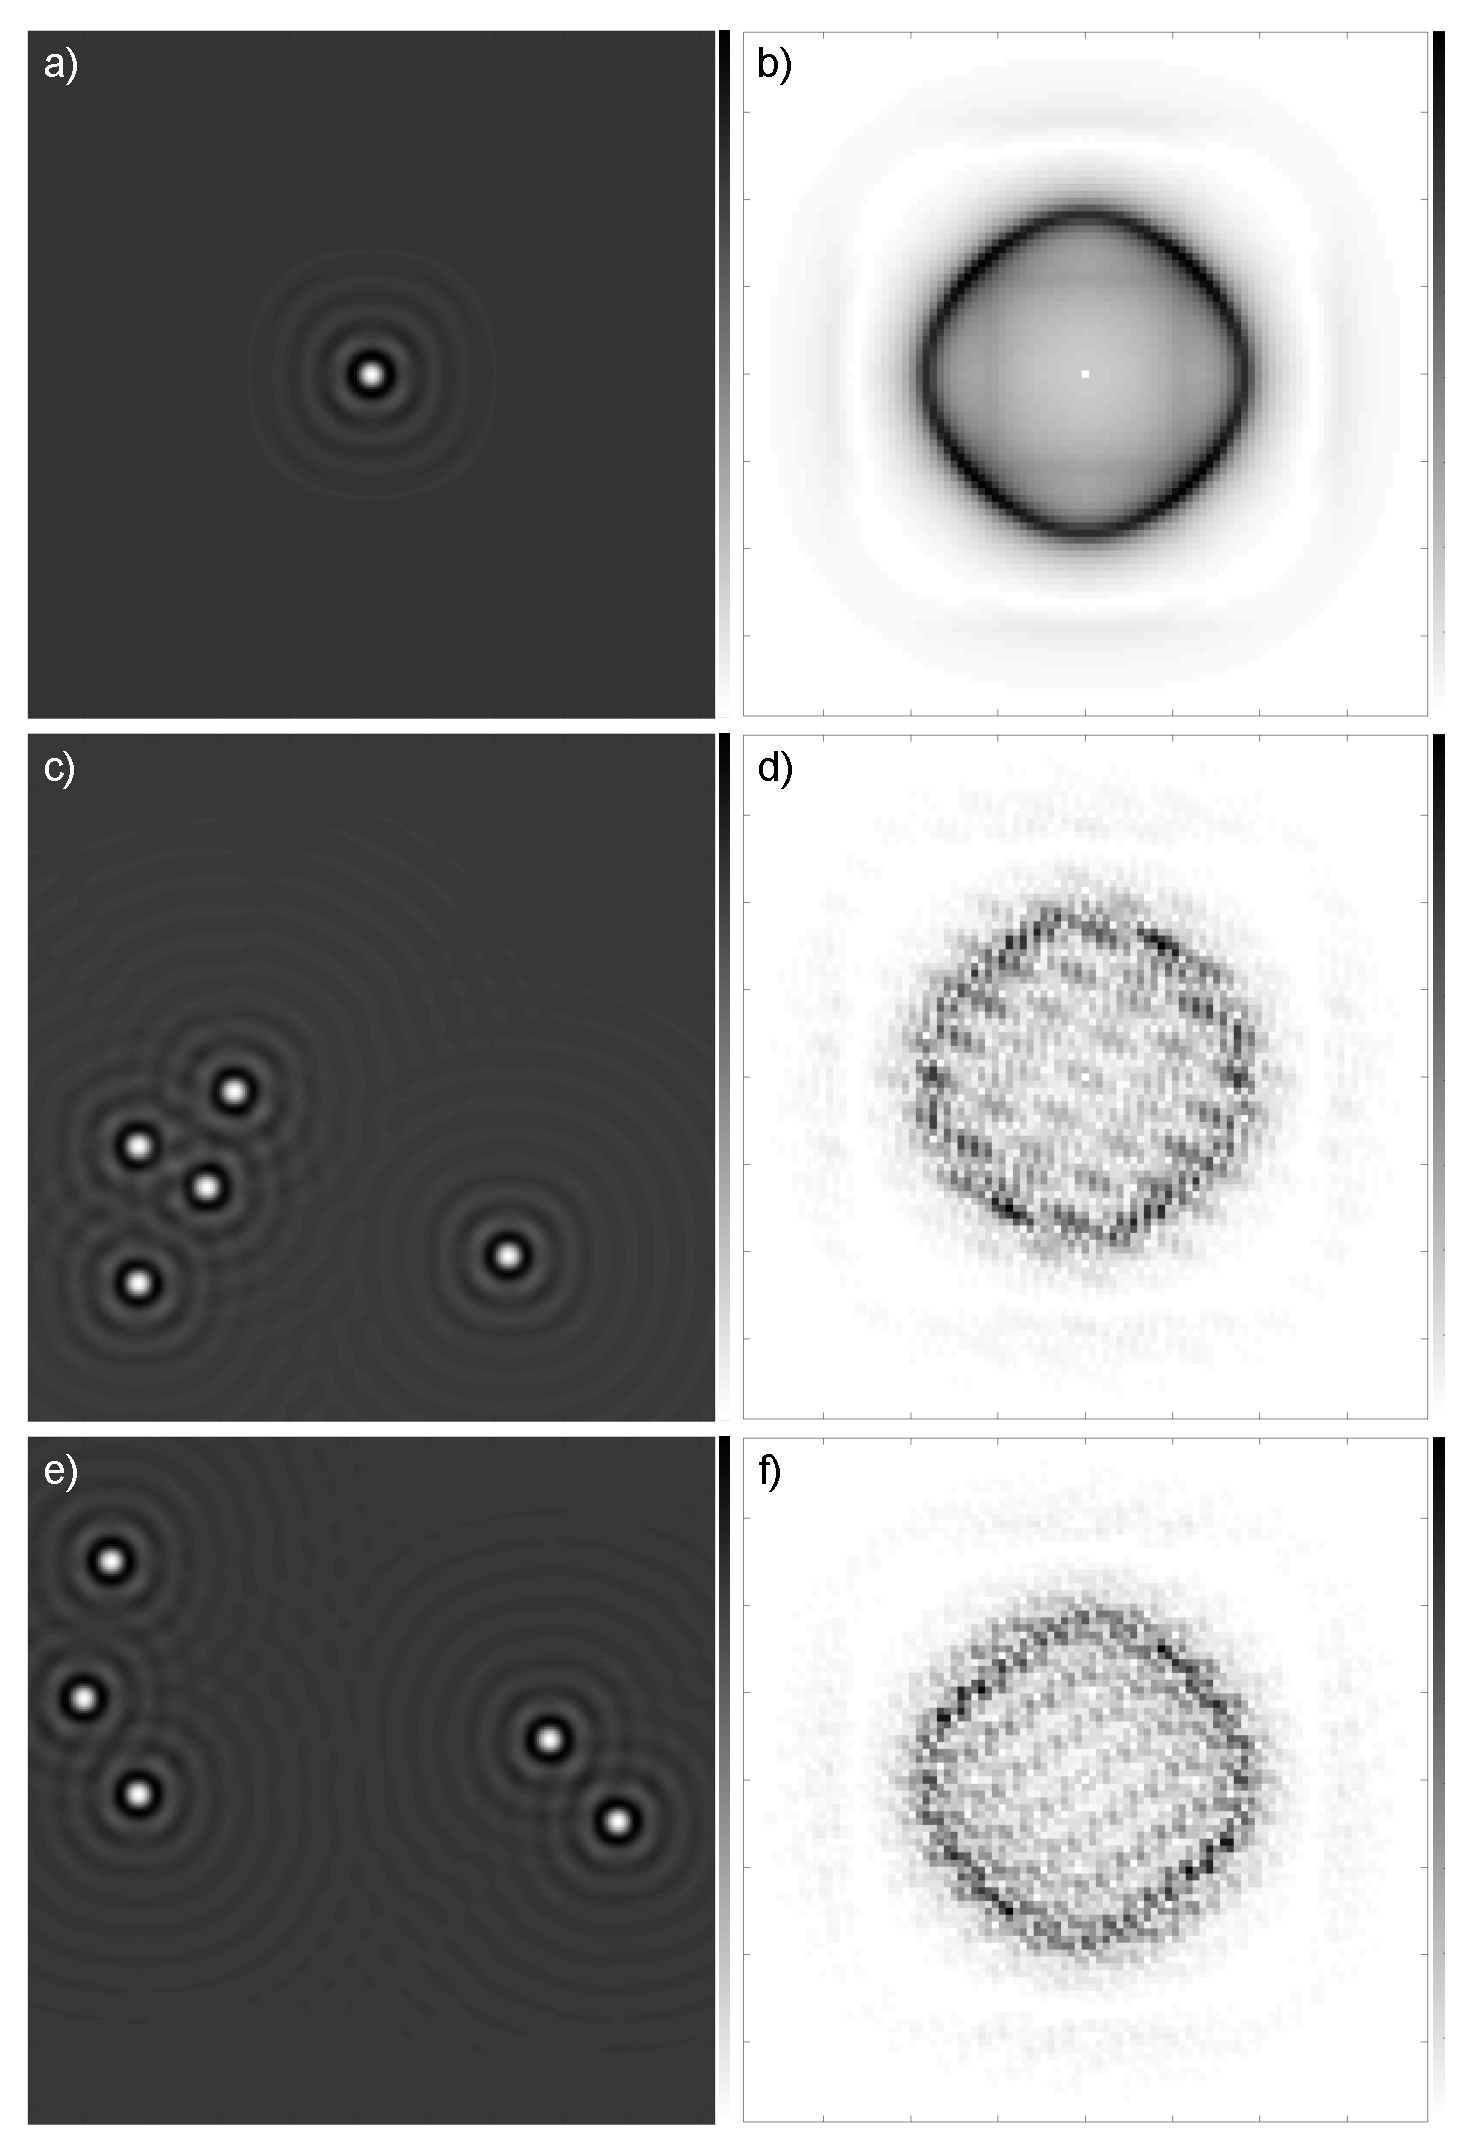
\includegraphics[width=0.85 \textwidth]{Ch5_phasenoise.pdf} 
	\centering
	\caption{Phase noise illustration. a),b): single defect scattering pattern and corresponding \textbf{q}-space QPI map. c)-f): multi-defect scattering with the same number of defects with different distributions, the corresponding QPI map presents phase noise with different patterns that associate with the defect distribution}
	\label{fig:ch5_phasenoise}
\end{figure}

Beyond the phenomenological illustration, we can further understand the source of phase noise with a mathematical analysis on multi-defect $\delta\rho(\textbf{x},\omega)$. We first discuss the form of the multi-defect T-matrix T, which is a $N_d \times N_d$ square matrix with entry T$_{\alpha \beta}$ representing the cross scattering term between defect m and n. We then separate the diagonal and off-diagonal terms and express T as\cite{leonard1972}:
\begin{align}
	\ T_{\alpha\beta} &= t_{\alpha} \delta_{\alpha\beta} + t_{\alpha} G_{0\alpha\beta} (1 - \delta_{\alpha\beta}) t_{\beta} + \sum_{\alpha' \neq \alpha, \beta} t_{\alpha} G_{0\alpha\alpha'} t_{\alpha'} G_{0\alpha'\beta} t_{\beta} + \cdots \label{eq_tmul}\\
	\label{eq.536}
	&= t_{\alpha} \delta_{\alpha\beta} + t_{\alpha} \sum_{\alpha'} \check{G}_{\alpha\alpha'} \ T_{\alpha'\beta},
\end{align}
\noindent where $t_{\alpha}$ is the T-matrix of a single impurity at site $\alpha$ and expressed on a matrix form in a localized basis set (i.e., expressed as the matrix with the same dimension as the multi-defect case but with only the $\alpha$'s diagonal entry none empty). And matrix $\check{G}_{\alpha\alpha'} = G_{0\alpha\alpha'}(1-\delta_{\alpha\alpha'})$, it contains the off-diagonal part of the Green's function. It has been shown by Fang et al. \cite{fangTheoryQuasiparticleInterference2013} that, in the Born approximation to the scattering amplitude, the first term dominates over the second term, and the latter can be omitted. We can, therefore, approximate multi-defect scattering with multiple single-defect scattering events. 

This approximation was then extended to the strong scattering case by Philipp et al. \cite{russmannInitioTheoryFourierTransformed2021}, under the assumption that the impurity concentration is low and the largest part of the surface is covered by pristine atoms and far from the impurities. They then utilized Equation \ref{eq.536} and further expressed the Green's function difference:

\[
\Delta G(\mathbf{r}, \mathbf{r}, E) = \int d^3 \mathbf{r}' \int d^3 \mathbf{r}'' \, G_0(\mathbf{r}, \mathbf{r}'; E) \, T(\mathbf{r}', \mathbf{r}''; E) \, G_0(\mathbf{r}'', \mathbf{r}; E)
\]

\begin{align}
	\label{eq.537}
	\Delta G_{\alpha \alpha} &= \Delta G^{(1)}_{\alpha \alpha} + \Delta G^{(2)}_{\alpha \alpha} \\
	\label{eq.538}
	&= \sum_{\alpha'} G_{0\alpha \alpha'} t G_{0\alpha' \alpha} + \sum_{\alpha'} G_{0\alpha \alpha'} t\sum_{\beta \beta'} \check{G}_{\alpha' \beta} \, T_{\beta \beta'} G_{0\beta' \alpha}.
\end{align}

\noindent By applying the stationary phase approximation \cite{lounisTheoryRealSpace2011} to $G_{0\beta'\alpha}$, and utilize the transnational symmetry of Bare lattice Green's function $G_0$, they showed:
\[
\Delta G^{(2)}_{\alpha\alpha}=\sum_{\alpha'}G_{0\alpha\alpha'}t\sum_{\beta\beta'}\check{G}_{\alpha'\beta}T_{\beta\beta'}K_{\beta'\alpha}e^{ik_{\beta'\alpha}\cdot R_{\beta'\alpha}},
\]
\noindent where the contribution of the last phase, $e^{ik_{\beta'\alpha}\cdot R_{\beta'\alpha}}$ can not be lifted, and is thus the source of the phase noise we observed in Fig. \ref{fig:ch5_phasenoise}. 

It is further noted that the contribution of the phase can be piratically canceled if we sum over all configurations of randomly distributed defects, which correspond to an infinitely large scanning surface, which can never be achieved. However, a decreased influence of this phase noise can be seen if we increase the density of the defects, as illustrated in Fig \ref{fig:ch5_changephasenoise}. This is because the patterns created by the phase noise become more fine-grained and can eventually be seen as featureless, similar to the random distribution of noise.  
%todo: verify whether this is true with more literature reviews. 

\begin{figure}
	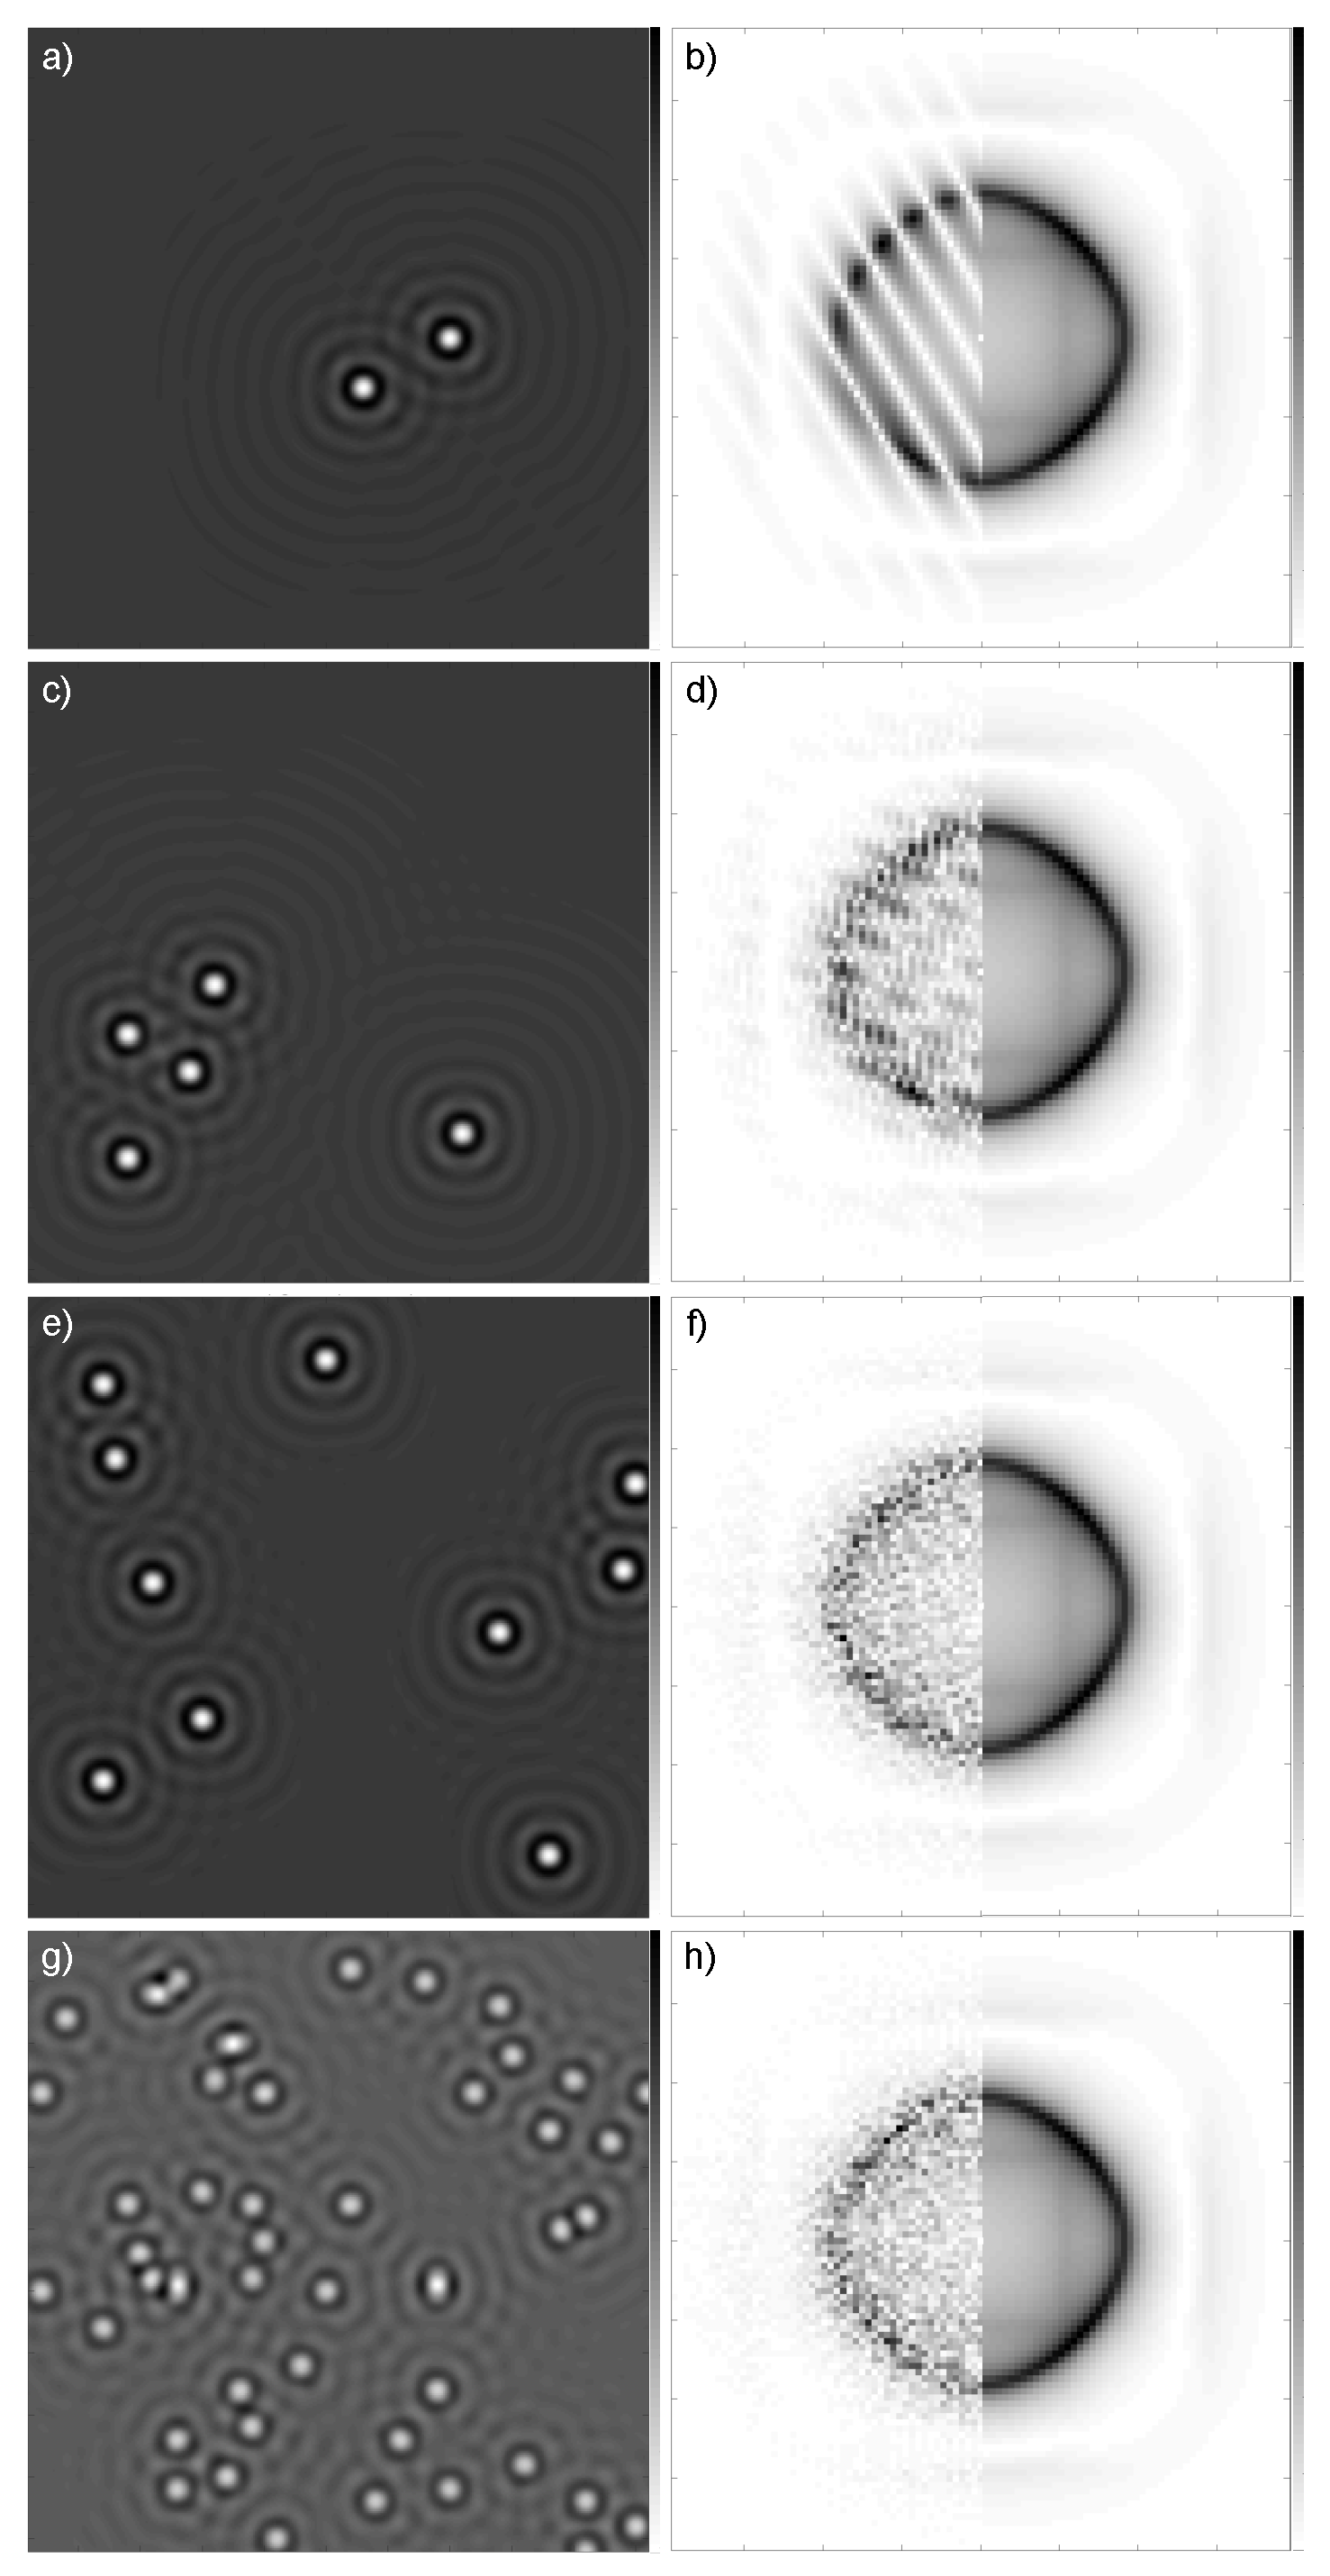
\includegraphics[width=0.7 \textwidth]{Ch5_changephasenoise.pdf} 
	\centering
	\caption{The effect of the phase noise is most prominent in the sparse defects regime. a)-h): $\delta\rho(\textbf{r},\omega)$ and \textbf{q}-space QPI plotted in pair with increasing defect concentration, showing the phase noise becomes more featureless. Single-defect QPI map is presented for reference on the right half of the \textbf{q}-space QPI.}
	\label{fig:ch5_changephasenoise}
\end{figure}

\section{A Multi-Channel Sparse Blind Deconvolution approach to STM}

In this chapter, we will introduce our approach to address the \ac{MC-SBD} problem. We will first analyze the bi-linear nature of \ac{MC-SBD}, and overview the possible methods that address it. We then briefly introduce the Riemannian Trust Region method (RTRM), a direct non-convex optimization algorithm that addresses the \ac{SBD} problem. Finally, we present our algorithm which extends \ac{RTRM} to multiple-channel cases. 

\ac{MC-SBD}, also known as the joint sparse blind deconvolution/demixing problem is a bi-linear problem, that is, the observed signal is modeled as a convolution (or equivalent linear operation) between pairs of two unknowns—and this operation is linear in each variable when the other is fixed, but not jointly linear. Bi-linear problems can be solved by either a lifted method or a direct method. A lifted method can formulate the initial bi-linear mapping of two unknowns to a linear mapping of a single unknown, by defining a one-to-one mapping from two unknowns to the targeted unknown. For example, given observation $y = \mathbb{A}(x,h)$, where $x \in \mathbb{R}^n$ and $h \in \mathbb{R}^m$ are two inputs we try to recover. We can define an outer product $X = xh^T\in \mathbb{R}^{n\times m}$, and rewrite observation $y = \mathbb{A'}(X)$. In the case of convolution, $\mathbb{A'}$ is the Lifted circular convolution operator. A lifted problem can be solved analytically, and since we are dealing with only one subspace defined by $X$, by assigning constraints on $(x,h)$,  $X$ usually present some internal structures, and we are left with a fully convex problem; thus, the convergence to global minimum can usually be proven, this is also known as the recovery guarantee. For example, Flinth et al. show that, given both inputs are sparse, they can achieve high probability recovery by lifting the \ac{MC-SBD} problem and applying a hierarchical sparsity framework[tocite]. 

However, in real cases, it is rare to find both inputs sparse. Moreover, the lifting method is normally computationally inefficient, as the dimension of output space is the product of two separate inputs, it expands quickly with higher input dimensions, making it unfavorable for larger size problems like the QPI-STM recovery, note that it is even more expensive in the multi-channel case, as now the dimension of output space is not only product of two input space but product of $2 \cdot types$ input spaces. On the contrary, a direct method updates one input while assuming the other one is fixed, the optimization space of the problem thus grows linearly with the input dimension. The trade-off is that with direct methods, recovery guarantee is hard to obtain, instead, local minimal recovery can be guaranteed with careful algorithm design. Local convergence can be combined with an initial guess that is close to the global minimum; this recipe of combining a good initial guess and an algorithm with strong guarantees of local convergence usually leads to good recovery. 

Our algorithm is a direct method that follows the above recipe, it utilizes Riemannian Trust Region Method(RTRM) to provide local convergence. Standard Trust Region Method is a second-order method that guarantees local minimum recovery, as long as the objective(ie, the cost function $\phi$) has no degenerate stationary points, that is, the Hessian $\Delta^2\phi$ has no zero eigenvalues. This ensures a sufficiently curved optimization landscape for the algorithm to make consistent progress. Moreover, compared to first-order methods based on gradient descent, Trust Region Methods has significantly faster convergences and a better overall tail convergence when the iterates are close to local minima. 

\ac{RTRM} is first raised by Absil et al. in 2007 as the extension of Trust Region Methods on a Riemannian sub-manifold, embedded in Euclidean spaces. This is advantageous since enforcing our manifold to follow certain geometry, for example in our case, we enforce the kernel to live on a hypersphere $S$ defined by Equation \ref{hypersphere}, which removes the scaling symmetry we discussed. As a result, the \ac{RTRM} provides strong guarantees that a local minimum of the objective be attained over S. We now present the \ac{RTRM} algorithm used by Cheung et al. \cite{cheungDictionaryLearningFouriertransform2020} that addresses \ac{SBD} problem; we then build on it and present our \ac{MC-SBD} algorithm. 

\subsection{SBD algorithm}
Recall we have the objective function $\phi_{\lambda}$: 
\begin{equation}
	\phi_{\lambda} = \frac{1}{2}\left\lVert A_0 * X_0 - Y \right\rVert^2_F + \lambda \cdot  \left\lVert X\right\rVert_1,
\end{equation}
since \ac{RTRM} is a second-order method, we need to make make our objective function smooth, more particular, we need to smooth the sparse regularizer. This can be achieved by approximate the $l_1-norm$ by $r_{\mu}(X)$:
\begin{equation}
	r_{\mu}(X) \equiv \sum_{i,j} \mu^2(\sqrt{1+\mu^{-2}\cdot X_{i,j}}-1), 
\end{equation}
this is called a pseudo-Huber regularizer, in the limit of $\mu -> 0$, the regularizar resembles $l_1-norm$, in our case, we choose $\mu = 10^{-6}$. 

To adopt a direct method as we discussed, we will updates each input to minimize the objective function while assuming the other input fixed. We now solve: 
\begin{equation}
	\label{sbdalgorithm}
	(\hat{A}, \hat{X}) \leftarrow \min_{{A} \in {S}} \left\{ 
	\phi_{\lambda}({A}) \equiv \min_{X} \left[ 
	\phi_{\lambda}({A}, {X}) \equiv \frac{1}{2} \left\| {A} * {X} - {Y} \right\|_F^2 
	+ \lambda \cdot r_{\mu}({X}) 
	\right] 
	\right\}.
\end{equation}
This updating algorithm consists of an inner and an outer solver. The inner solver: $X \leftarrow \mathbf{XSolve}(A, \lambda)$, that is, obtaining $\hat{X}$ that minimizes $\phi_{\lambda}(A,X)$ using \ac{RTRM}. The outer solver: $A \leftarrow \mathbf{ASolve}(A, \hat{X}, \lambda)$, updating $A$ that minimizes $\phi_{\lambda}(A,X)$ using \ac{RTRM}. Since $\mathbf{XSolve}$ is an intermediate step, for $i^{th}$ iteration, we can simply write the process as: $(A^{i+1}, X^{i+1}) \leftarrow \mathbf{ASolve}(A^{i}, X^{i}, \lambda; Y,(m_1,m_2))$, where $(m_1,m_2)$ is the predefined kernel size. Or for a complete process of in total n such loops, we write $(A, X) \leftarrow \mathbf{ASolve}^n(A, X, \lambda; Y,(m_1,m_2))$

We can then write the Complete SBD-STM procedure: 

\begin{algorithm}
	\label{SBDalgo}
	\caption{Complete SBD-STM Procedure}
	\textbf{Input:}
	\begin{itemize}
		\item Observation $Y \in \mathbb{R}^{n_1 \times n_2 \times s}$,
		\item Kernel size $(m_1, m_2)$,
		\item Initial $\lambda_0 \geq 0$, decay rate $\alpha \in [0,1)$, and final $\lambda_{\text{end}} \geq 0$.
	\end{itemize}
	
	\textbf{Phase I:}
	\begin{enumerate}
		\item Randomly initialize: $A^{(0)} \in S = \mathbb{S}^{m_1 \times m_2 \times s}$.
		\item $A_\star^{(0)} \leftarrow \texttt{ASolve}^N(A^{(0)}, \lambda_0, loop)$.
	\end{enumerate}
	
	\textbf{Phase II:}
	\begin{enumerate}
		\item Lifting: Get $A^{(1)} \in S' = \mathbb{S}^{m_1' \times m_2' \times s}$ by zero-padding the edges of $A_\star^{(0)}$ with a border of width $\left\lfloor \frac{m_1}{2} \right\rfloor$.
		\item Set $\lambda_1 = \lambda_0$.
		\item Refinement: \textbf{Repeat} for $k = 1, 2, \dots$ \textbf{until} $\lambda_k \leq \lambda_{\text{end}}$,
		\begin{enumerate}
			\item[(a)] $A_\star^{(k)} \leftarrow \texttt{ASolve}^N(A^{(k)}, \lambda_k)$,
			\item[(b)] \textbf{Centering}:
			\begin{enumerate}
				\item[i.] Find the size $m_1 \times m_2$ submatrix of $A_\star^{(k)}$ that maximizes the Frobenius (square) norm across all $m_1 \times m_2$ submatrices.
				\item[ii.] Get $A^{(k+1)}$ by shifting $A_\star^{(k)}$ so that the chosen $m_1 \times m_2$ restriction is in the center, removing and zero-padding entries as needed.
				\item[iii.] Normalize $A^{(k+1)}$ so it lies in $S'$.
			\end{enumerate}
			\item[(c)] Set $\lambda_{k+1} = \alpha \lambda_k$.
		\end{enumerate}
	\end{enumerate}
	
	\textbf{Output:}
	\begin{itemize}
		\item Extract $\hat{A} \in S$ by extracting the restriction of the final $A^{(k+1)}$ to the center $m_1 \times m_2$ window.
		\item Find the corresponding activation map $\hat{X} \in \mathbb{R}^{n_1 \times n_2}$ by solving $\min_{X} \psi_{\lambda_k}(\hat{A}, X)$.
	\end{itemize}
\end{algorithm}

The kernel $A^{(0)}$ is first randomly initialized and normalized, it is then fed into two phases sequentially. Both phases utilize the same core algorithm $\mathbf{ASolve}$ as described above. Phase I aims to obtain a primary kernel $A^{(0)}_*$ given $\lambda_0$. Phase II serves as a refinement that increases the recovery quality by applying a stricter sparsity regularizer $\lambda_{k} > \lambda_0$, as well as addresses the degeneracy brought by the translation symmetry formulated in Equation \ref{translational_symm}. The latter is achieved by applying a so-called shift-truncate method, as illustrated in Figure. \ref{fig:ch6_phase2}. This method lifts the primary kernel $A^{(0)}_*$ by zero padding its edge with zeros to get a padded kernel with bigger size $(m_1',m_2')$, the padded kernel is then fed into $\mathbf{ASolve}$ with stricter $\lambda_{k}$ and get $A^{(k)}_*$ as shown in b). The Frobenius square norms are calculated on all the possible submatrices with size $(m_1,m_2)$ within $A^{(k)}_*$. An example of the submatrix window is illustrated in red square in b), and we can generate a heat map as shown in c), with each pixel in the heat map corresponding to a submatrix. The algorithm then finds the submatrix that maximizes the norm, which corresponds to the red cross in c), and we then truncate according to this submatrix and normalize it to get $A^{(k+1)}$. 

Using the Frobenius square norm score in the shift-truncate method is common practice and works well in most cases. However, it fails in more complicated situations, especially when we have other features in the padded kernel, this is illustrated in Figure. \ref{fig:ch6_phase2mod}, given primary kernel $A^{(0)}_*$, we pad it and apply $\mathbf{ASolve}$ to get $A^{(1)}_*$. The Frobenius square norm score is shown in c) and by picking the maximum, we get e), which resembles the primary kernel. This issue is mainly due to faint features around the primary feature. We can improve this algorithm by applying a radial decay term $\eta_d(r) = e^{-lnd \cdot r}$ to the Frobenius square norm, where r is the normalized distance from the submatrix window center, and d is the tunable decay factor. This biases the center features and is consistent with the decaying nature of the QPI patterns. With this decay term (d=2) applied, we obtain a heat map $S'$ as shown in d), and a truncated kernel $A^{(1)'}$ in f) has the primary more centered compared to e). For convenience, unless otherwise mentioned, all phase II that we introduced later will be using the center-biased Frobenius square norm. 

\begin{figure}
	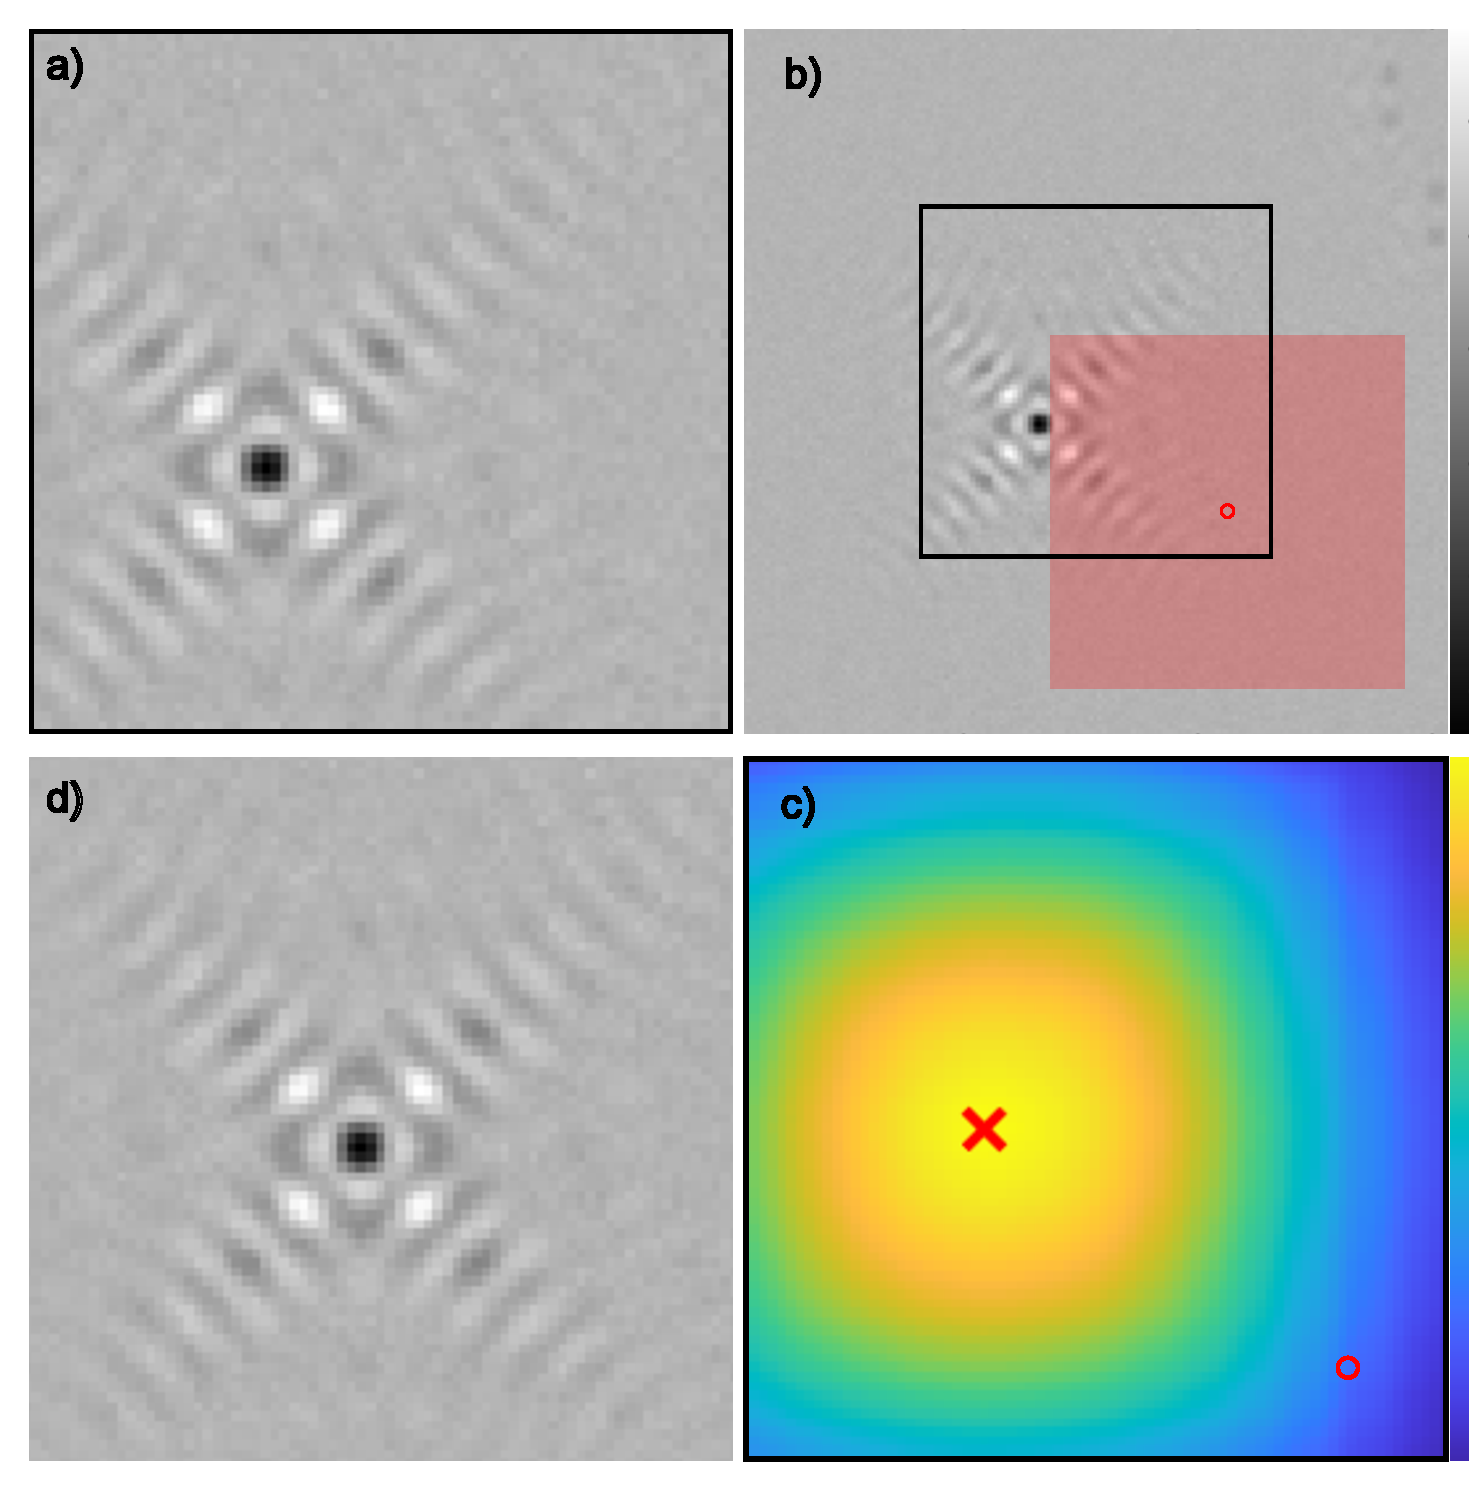
\includegraphics[width= \textwidth]{phase2old.pdf}
	\centering
	\caption{}
	\label{fig:ch6_phase2}
\end{figure}


\begin{figure}
	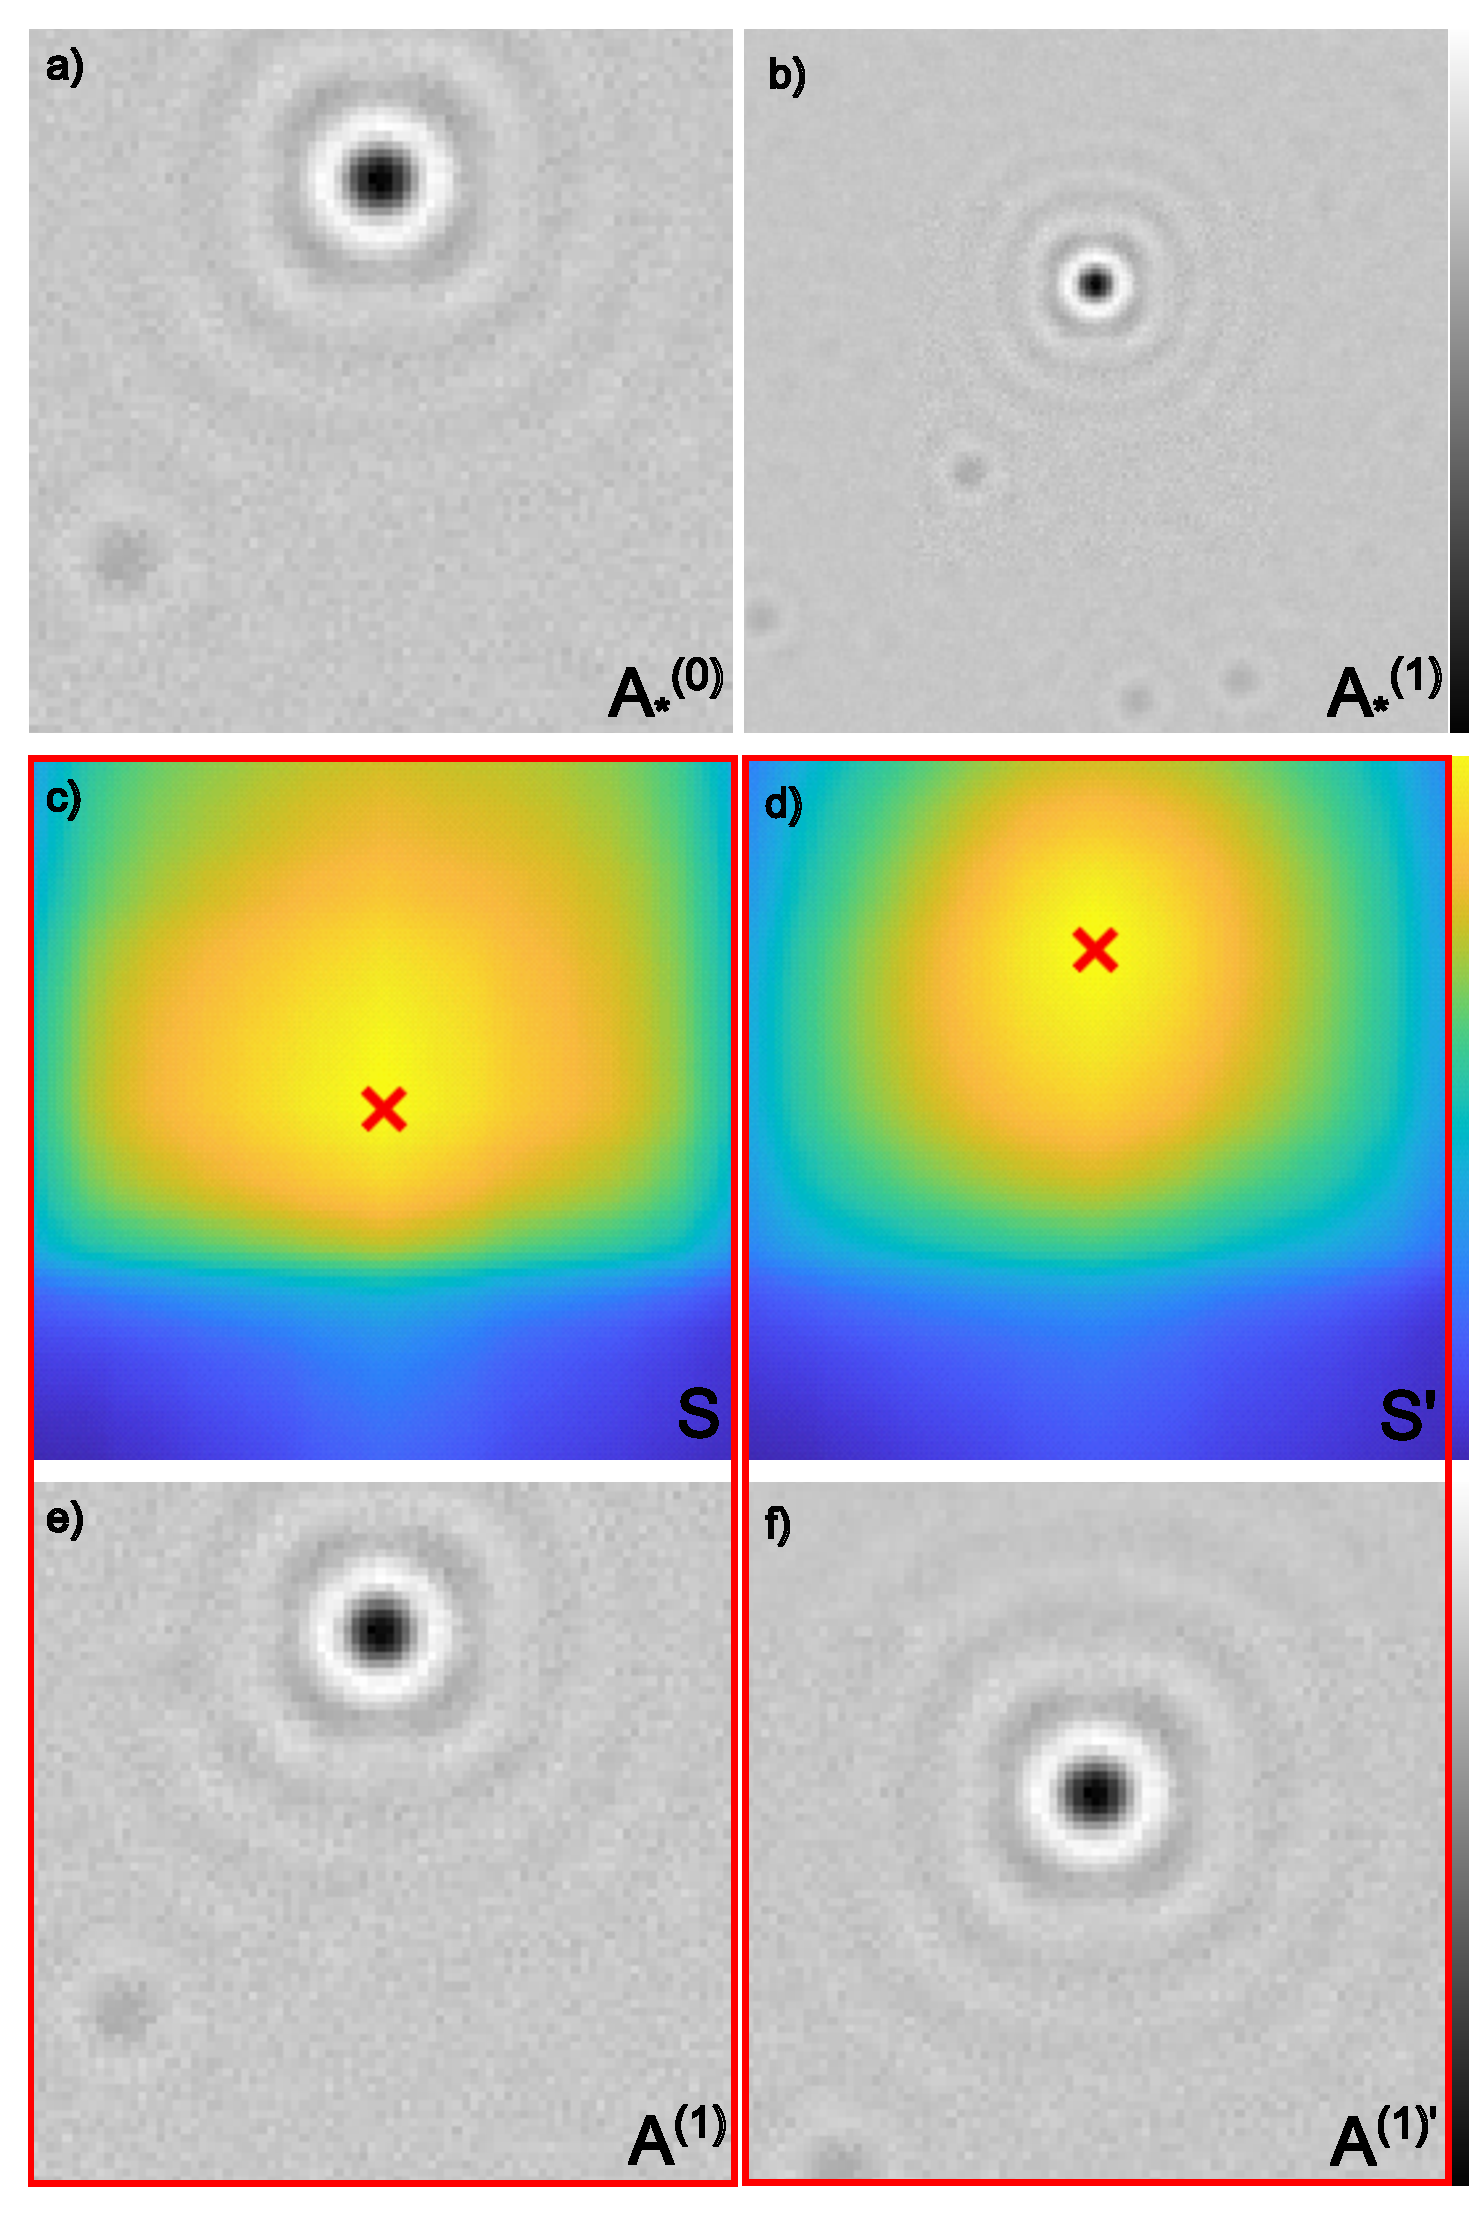
\includegraphics[width= \textwidth]{phase2mod.pdf}
	\centering
	\caption{}
	\label{fig:ch6_phase2mod}
\end{figure}


\subsection{MC-SBD algorithm}
We first establish some intuition about the multi-channel blind deconvolution process. Consider a generation process of the observation $Y$: 
\begin{equation}
	\label{eq:dec}
	Y = \sum_{i}^{s} A_i^{gt} * X_i^{gt} + noise, 
\end{equation}
\noindent where the superscript $gt$ indicate the ground truth. \ac{MC-SBD} aims to deconvolute multiple kernel-activation pairs given observation $Y$, such that $A_i=A_i^{gt}$ and $X_i = X_i^{gt}$, for all types $i \in [1,2,...,s]$. We can rewrite Equation \ref{eq:dec} as: 
\begin{align}
	Y &= \sum_{i}^{s} Y_i^{gt} + noise,\\ 
	Y_i^{gt} &= A_i^{gt} * X_i^{gt}.
\end{align}
\noindent This hints at the two separate operations in the data generation process: convolution and composition. Therefore, our \ac{MC-SBD} follows the reverse order: we first decompose the observation into kernel-specific components and then deconvolute each component into its kernel and activation. 

Due to the two-stage nature of the process, we adopt a hierarchical direct treatment across both the intra-type and the inter-type levels. At the intra-type level, when updating a specific kernel $A_j$, we hold its corresponding activation $X_j$ fixed -- a strategy inherited from the single-type \ac{SBD} algorithm. At the inter-type level, when handling the $j$-th type, we treat all $Y_i, i\neq j$ as fixed. 

This hierarchical approach enables isolated analysis for each type’s recovery:
\begin{align}
	Y_j &= Y - [\sum_{i\neq j}Y_i + noise],\\
	A_j * X_j &= Y - [\sum_{i\neq j}Y_i + noise].
\end{align} 
\noindent We can then write $Y_i = Y_i^{gt}- Y_i^{residual}$ and substitute the observation with \ref{eq:dec}. Then we have:
\begin{align}
	A_j * X_j &= \sum_{i}^{s} Y_i^{gt} + noise' - [\sum_{i\neq j}(Y_i^{gt}- Y_i^{residual}) + noise],\\ \label{eq:622}
	A_j * X_j &= Y_j^{gt}+ \sum_{i\neq j}Y_i^{residual} + noise = Y_j,
\end{align} 

\noindent The combined noise terms are absorbed into a single term. Equation \ref{eq:622} now resembles a single blind deconvolution problem, which can be addressed using the \ac{SBD} algorithm.

Smaller $Y_i^{residual}$ values for all $i \neq j$ lead to better-posed subproblems for each type. Consequently, when updating with the \ac{SBD} algorithm, we can produce a result $Y_j = A_j* X_j$ that is closer to the true component $Y_j^{gt}$. This motivates a loop structure in our algorithm: by updating one type (e.g. $j$), we reduce its residual $Y_j^{residual}$, which in turn helps improve the subsequent recovery of another type $i \neq j$. Through iterative refinement, given the local convergence guarantees provided by the \ac{RTRM} method, the residuals across all types could be gradually minimized, allowing the full reconstruction to converge towards the ground truth. However, this logic can break down in the early stages of optimization, where the residuals are large and noisy—making it difficult for the algorithm to enter a reliable refinement path. To address this challenge, we designed specific strategies that guide the optimization toward stability and correctness during these critical initial steps.

A complete description of the \ac{MC-SBD} algorithm is presented in Algorithm \ref{MTSBDalgo}; it preserves the two-phase structure from the original \ac{SBD} method. Apart from the loop structure discussed above, two important strategies are worth noting. 

First, The blending strategy is a dynamic weighting mechanism that constructs an effective observation for each kernel by combining the current residual with the global reconstruction: 
\begin{equation}
	Y_i = Y_{res} + \left(1-\frac{1}{\beta t+1}\right)A_i * X_i + \frac{1}{\beta t+1}Y_{sum},
\end{equation}
\noindent where $Y_{sum} = \sum_{j=1}^s A_j * X_j$ represents the sum of all convolution pairs, and the blending factor $\beta > 0$ controls the rate at which the influence of other components decreases over iterations.

This approach is particularly important in the early stages of decomposition, where the residuals are large and noisy. Without blending, directly updating each kernel-activation pair using such corrupted residuals can lead to poor local minima and error accumulation across iterations. By using a blending factor $\beta$ to control the mixing ratio over time, the algorithm initially relies more on the global structure to stabilize updates and gradually shifts toward using the true residual as the decomposition improves. This smooth transition prevents the algorithm from veering off due to early missteps and guides it toward more reliable solutions.

Another strategy is the variance-based update ordering, it prioritizes kernel updates according to the magnitude of their kernel variance, processing high-variance components first. This ordering is crucial because the residual is updated sequentially after each kernel is refined, meaning earlier updates have a greater influence on the remaining residual. By addressing the most dominant structures in the data first, the algorithm quickly reduces the residual and improves the signal quality for the weaker components updated later. This leads to better-conditioned subproblems throughout the iteration and helps avoid cumulative distortion that could arise from poor early updates to minor components.

\begin{algorithm}
	\label{MTSBDalgo}
	\caption{Multi-Type SBD-STM Procedure}
	\textbf{Input:}
	\begin{itemize}
		\item Observation $Y \in \mathbb{R}^{n_1 \times n_2}$,
		\item Kernel size list $k \in \mathbb{R}^{s \times 2}$ for $s$ kernels,
		\item Initial $\lambda_{1,i} \geq 0$, and final $\lambda_{2,i} > \lambda_{1,i}$, for $i=1,\dots,s$.
		\item Border padding $k_{plus} \in \mathbb{R}^{s \times 2}$.
		\item Faint factor $\beta > 0 $ for demixing.
	\end{itemize}
	
	\textbf{Phase I:}
	\begin{enumerate}
		\item Initialize kernels $A^{(0)}_i \in \mathbb{R}^{k_i}$ for $i=1,\dots,s$
		\item Initialize activation
		\item For each global iteration $t=1,\dots,T$:
		\begin{enumerate}
			\item Compute residual: $Y_{res} = Y - Y_{sum}$; $Y_{sum} = \sum_{j=1}^s A_j * X_j$
			\item For each kernel $i$ in descending order of variance:
			\begin{enumerate}
				\item Set up $Y_{i} = Y_{res} + (1-\frac{1}{\beta t+1})A_i * X_i + \frac{1}{\beta t+1}Y_{sum}$
				\item Update $(A_i, X_i) \leftarrow \texttt{ASolve}^N(Y_{i}, A_i, \lambda_{1,i})$
				\item Update residual: $Y_{res} = Y_{i} - A_i * X_i$
			\end{enumerate}
		\end{enumerate}
	\end{enumerate}
	
	\textbf{Phase II:}
	\begin{enumerate}
		\item Lifting: For each kernel $i$:
		\begin{enumerate}
			\item Create $A^{(1)}_i \in \mathbb{R}^{k_i + 2k_{plus}}$ by zero-padding $A^{(0)}_i$ around the edge. 
		\end{enumerate}
		\item For each refinement $r=1,\dots,R$:
		\begin{enumerate}
			\item For each kernel $i$ in order:
			\begin{enumerate}
				\item $\lambda_i = \lambda_{1,i} +\frac{r}{R}(\lambda_{2,i}- \lambda_{1,i})$
				\item Set up $Y_{i} = Y_{res} + A_i^{(r)} * X_i^{(r)}$
				\item Update $(A_i^{(r+1)}, X_i^{(r+1)}) \leftarrow \texttt{ASolve}^N(Y_{i},  A_i^{(r)}, \lambda_i)$
				\item \textbf{Centering}:
				\begin{enumerate}
					\item Calculate score $s(\tau)$, the center-biased Frobenius (square) norm on the submatrices with every possible shift $\tau$.
					\item Find shift $\tau^*$ maximizing $s(\tau)$
					\item Shift kernel by $\tau^*$ and activation map by $-\tau^*$
				\end{enumerate}
				\item Update residual: $Y_{res} = Y_{i} - A_i^{(r+1)} * X_i^{(r+1)}$
			\end{enumerate}
		\end{enumerate}
	\end{enumerate}
	
	\textbf{Output:}
	\begin{itemize}
		\item Final kernels $\hat{A}_i \in \mathbb{R}^{k_i}$ extracted from center of padded kernels
		\item Calculate activation maps $\hat{X}_i \in \mathbb{R}^{n_1 \times n_2}$ with \texttt{XSolve}
	\end{itemize}
\end{algorithm}







